\section*{木の場合}

{\graphStar}を一般化した地図の形状として木を考えることができる.
{\graphStar}のときと同様,木の各葉のみに{\maxIdletime}が定められているとする.
長さが$0$の辺を許せば,任意の木はその葉どうしの距離を保ったまま二分木に変換できるので,
本節では二分木の地図を{\graphTree}と呼び,
{\graphTree}の場合の{\PPProfit}について考える.

Coeneら\cite{coene2011charlemagne}は{\independentPP}を地図が{\graphTree}の場合について調べている.
{\independentPP}においては,巡査が一人かつ全点の利得と{\maxIdletime}が等しい場合は,地図が{\graphTree}であっても多項式時間で解ける\cite[Corollary~3]{coene2011charlemagne}のに対し,
巡査数,利得,{\maxIdletime}のいずれか一つでも一般の場合は{\graphStar}であってもNP困難である\cite[Theorems 5, 6 and 10]{coene2011charlemagne}.
巡査が一人の場合は{\PPProfit}と{\independentPP}は同じ問題であるから,
{\graphTree}で全点の利得と{\maxIdletime}が等しいときは多項式時間で解くことができ,
利得か{\maxIdletime}のいずれかが一般の場合はNP困難であることは直ちにいえる.
しかし,巡査数が一般で全点の利得と{\maxIdletime}が等しい場合は,
{\PPProfit}では
地図が{\graphStar}のときは多項式時間で解けるので,{\graphTree}でどうなるかは未解決である.

\newcommand{\separatedPatroll}{左右独立運行}
\newcommand{\cooperativePatroll}{全員協力運行}


我々はまず,星ではない二分木の例として
図\ref{figure: twoStarsTree}左のような例を考えた.
\begin{figure}
  \centering
  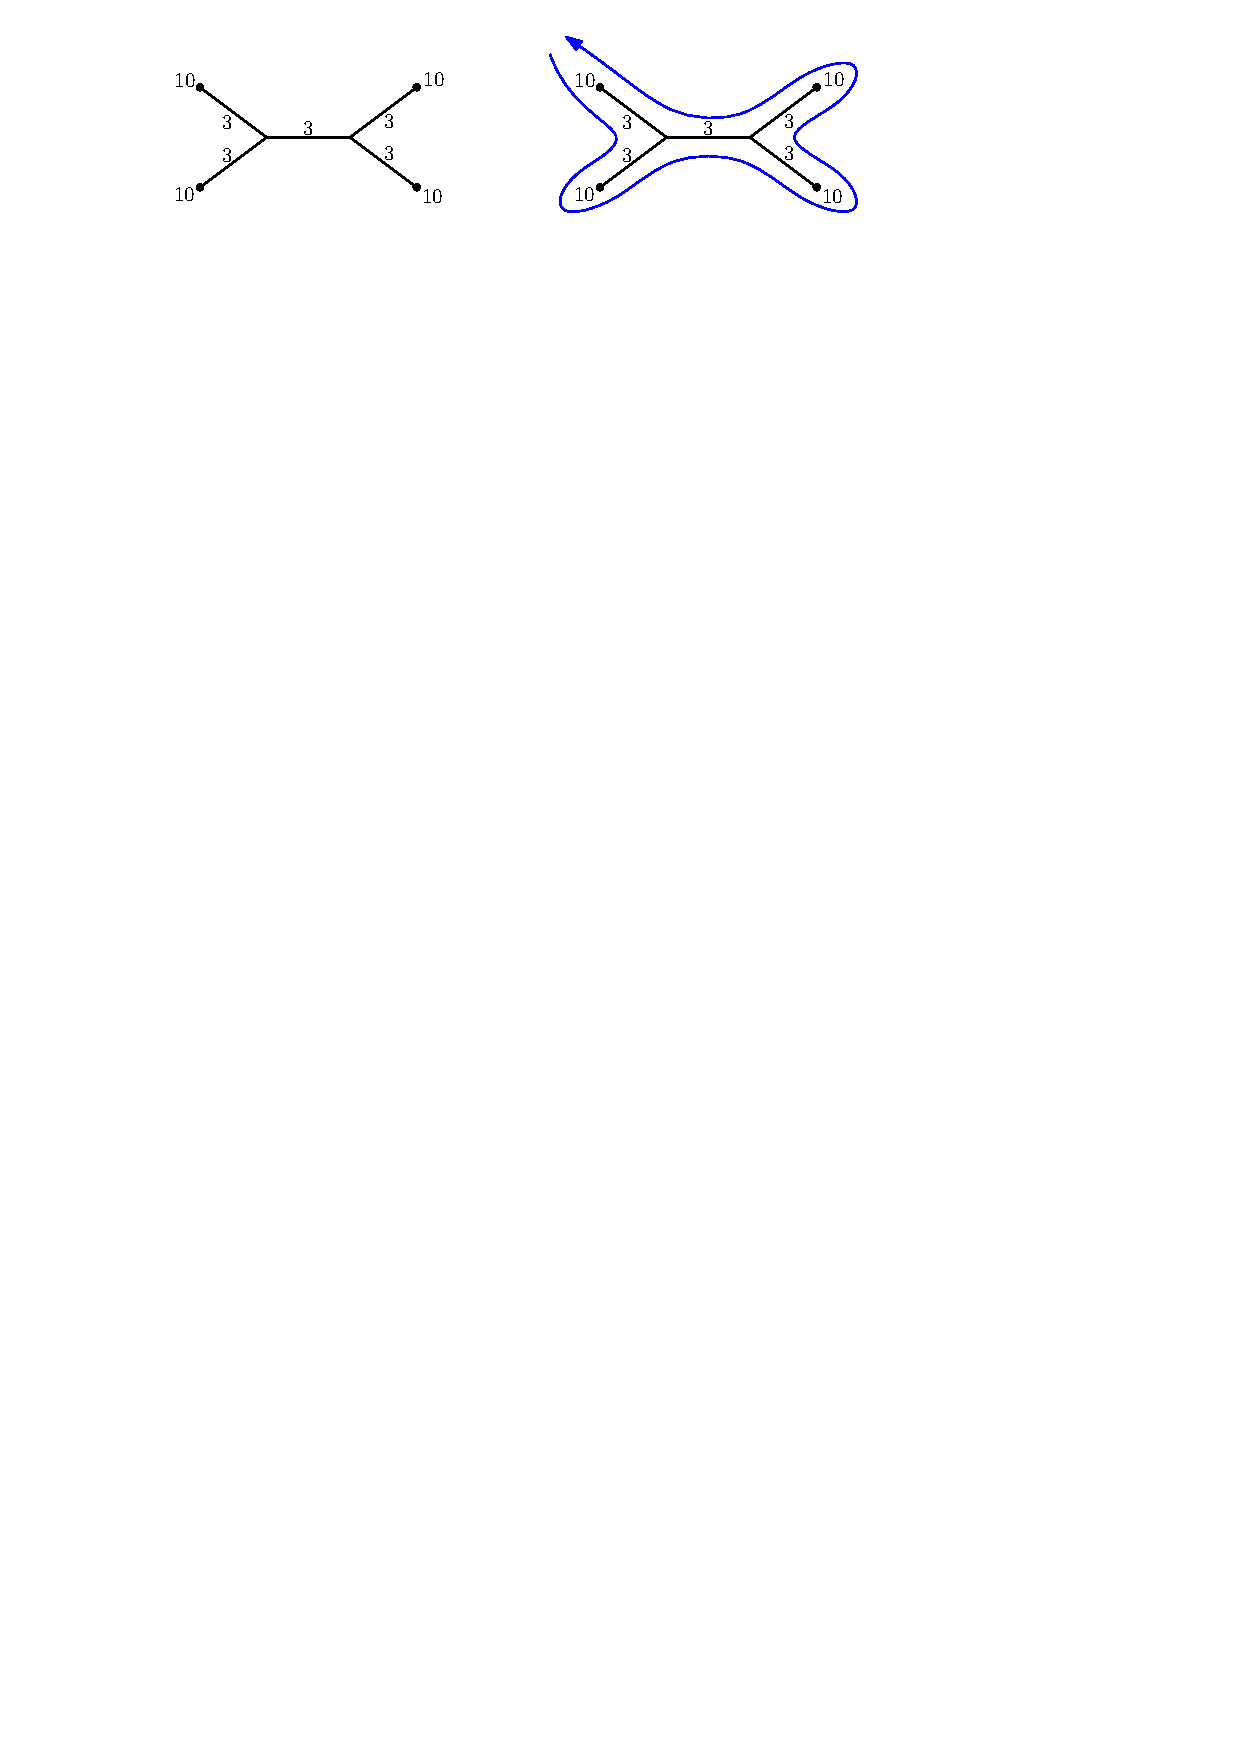
\includegraphics[scale=1.0]{\figdir/tree.pdf}
  \caption{
    $2$点からなる星二つを橋でつないだ木.
    点と辺に書かれた数は,それぞれ{\maxIdletime}と距離である.
    それぞれの星は補題\ref{lemm:StarConditionOfGuarding}から
    全点警邏に二人ずつの巡査を要する.
    一方,図のような順路の周回を行うとき
    1周にかかる時間は$30$であり,
    $3$人の巡査が時間$10$ずつずれてこの周回を行うと
    各点はちょうど時間$10$ごとに訪問される.
    よって,この例では全員協力運行の方が少ない人数で全点を警邏できる.
  }
  \label{figure: twoStarsTree}
\end{figure}
図\ref{figure: twoStarsTree}左の例では,2点からなる二つの星の中心どうしが一本の橋で結ばれている.
ここで,この{\graphTree}の地図の全点警邏に必要な最小の巡査数を考えてみる.
%
まず,左右の星を独立に{\graphStar}に対する最適戦略で警邏する運行が考えられる.これを\defword{\separatedPatroll}と呼ぶことにする.
補題\ref{lemm:StarConditionOfGuarding}から
星それぞれは全点警邏に2人,合計$4$人の巡査を要することが分かる.
%
一方,
図\ref{figure: twoStarsTree}右のような巡回を繰り返す運行を
$3$人の巡査が{\maxIdletime}$10$ずつずれて行うと全点を警邏できる.
このように巡査全員が全体を一度ずつ訪問する巡回を繰り返す運行を\defword{\cooperativePatroll}と呼ぶことにする.
図\ref{figure: twoStarsTree}左の例には存在しないが,隣接辺が$q/2$より長い点が存在する場合は{\cooperativePatroll}では巡査が一人停止して担当するものとする.

この例で仮に橋の長さが$10$などとしてみると,
全員協力運行では$3$人の巡査では全点警邏ができなくなり,
巡査$4$人による{\separatedPatroll}が最小人数の運行となる.
このように,橋の長さによって橋を渡るべきかどうかが変わる.

より一般に二つの星とその中心間を結ぶ長さ$b$の橋からなる{\graphTree}の地図$T$について考える.
左右の星の点集合をそれぞれ$L, R$とする.
全点の{\maxIdletime}を$q$とする.
また,以下では$S_V := \sum_{v \in V} \min(2d_v, q)$と書くことにする.
\newcommand{\lrceil}[1]{\lceil{#1}\rceil}

{\separatedPatroll}では,補題\ref{lemm:StarConditionOfGuarding}より,
左の星の全点警邏に$\lrceil{S_L / q}$人,
右の星の全点警邏に$\lrceil{S_R / q}$人の巡査を要する.
全員協力運行では$T$全点の警邏に
$\lrceil{( 2b + S_{L \cup R} ) / q}
 = \lrceil{( 2b + S_L + S_R ) / q}$%
人の巡査を要する.
よって,$T$は多くとも
$\min(
  \lrceil{( 2b + S_L + S_R ) / q},
  \lrceil{S_L / q} + \lrceil{S_R / q} )$%
の巡査で警邏できる.

$T$の橋の長さを$0$にした地図を$T'$とすると,
$T'$全体は点集合が$L \cup R$の{\graphStar}となり,
全点警邏には$\lrceil{(S_L + S_R) / q}$人の巡査が必要である.
$T'$の全点警邏に必要な最小巡査数は明らかに$T$の全点警邏に必要な最小巡査数以下となるので,
$T$の警邏には少なくとも$\lrceil{(S_L + S_R) / q}$人の巡査が必要である.

以上より,$T$の全点警邏に必要な巡査の最小数を$m_{\rm min}$と書くと,
\[
  \lrceil{(S_L + S_R) / q}
    \leq m_{\rm min}
    \leq \min(
        \lrceil{( 2b + S_L + S_R ) / q},
        \lrceil{S_L / q} + \lrceil{S_R / q} )
\]
となる.
我々は
$m_{\rm min} = \min(
        \lrceil{( 2b + S_L + S_R ) / q},
        \lrceil{S_L / q} + \lrceil{S_R / q} )$,
即ち,{\separatedPatroll}か{\cooperativePatroll}のいずれかは最適であると予想しているが,これを示すことはできていない.

なお,図\ref{figure: twoStarsTree}の例では
$\lrceil{(S_L + S_R) / q} = 3$であるので
全員協力運行は最小人数で全点警邏を行う戦略であることが分かる.

% \begin{itemize}
%   \item 運行の帰着で示すのが難しそう(仮説の運行は複数人の動きを同時に決めているので).
%   \item 1度も橋を渡らない運行では左右独立運行が最適.
%   \item 全点警邏可能かどうかの判定すら多項式時間でできるか未解決
% \end{itemize}
